\section{Билет 31.  Понятие правильной нормальной производной. Существование правильной нормальной производной у потенциала простого слоя с непрерывной плотностью Формула скачка для нормальной производной}
Мотивация: во внутренней задаче Неймана (билет 14) ищется решение $u(x) \in C^2(\Omega) \cap C^1(\bar{\Omega})$ уравнения $$\Delta u = f(x), x \in \Omega$$ при условии $$\frac{\partial u}{\partial \vec{n}}|_r = u_1(x),$$ где $u_1 \in C(\Gamma)$.

Но существуют примеры гармонических в области функций, градиент которых нельзя продолжить по непрерывности на замыкание этой области. Можно расширить понятие классического решения.

Пусть $u(x) \in C^1(\Omega) \cap C(\bar{\Omega}), \Omega$ - ограниченная область в $\R^3$ с границей $\Gamma \in C^2$
\begin{center}
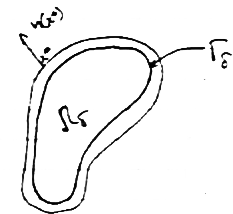
\includegraphics[width=0.2\textwidth]{31_1_new}
\end{center}
Пусть $x^o \in \Gamma$, а $\vec{n(x^o)}$ - нормаль к $\Gamma$ в $x^o$ Т.к. $\Gamma \in C^2$, $\vec{n(x^o)}$ - непрерывная функция по $x^o$. Проведем через $x^o$ прямую $x = x^o + \vec{n(x^o)}t, t \in \mathbb{R}$

Распишем произведенеие $$(\vec{n}(x^o), \triangledown u) = \sum_{k=1}^{3} n_x(x^o)\frac{\partial u}{\partial x_k}(x) = \frac{du(x^o + \vec{n}(x^o)t)}{dt} = \frac{\partial u}{\partial \vec{n}(x^o)}$$

\begin{definition}
Говорят, что $u(x)$ имеет \textbf{правильную нормальную производную} по направлению внешней нормали на $\Gamma$ из $\Omega$, если  
\begin{enumerate}
\item $\forall x^o \in \Gamma$ существует конечный предел 
$$\frac{\partial u}{\partial \vec{n}}(x^o) \equiv \lim_{x = x^o + \vec{n}(x^o)t,\\ x \in \Omega, \\ x \to x^o} \frac{\partial u}{\partial \vec{n}(x^o)}(x)$$

\item Этот предел равномерный по $x^o \in \Gamma$
\end{enumerate}
\end{definition}
\begin{lemma}
Если u(x) имеет ПНП по нормали $\vec{n}(x^o)$ из $\Omega$ на $\Gamma$, то 
\begin{enumerate}
\item u(x) имеет обычную производную по нормали $\vec{n}(x^o)$ в точке $x^o \in \Gamma$, и эта производная совпадает с ПНП 

\item ПНП $\in C(\Gamma)$
\end{enumerate}
\end{lemma}
\begin{proof} Обычная производная по нормали $$\lim_{x \to x^o, x = x^o + \vec{n}(x^o)t} \frac{u(x^o) - u(x)}{|x^o - x|} = \lim_{t < 0, t \to 0} \frac{u(x^o - u(x^o + \vec{n}(x^o)t))}{-t} = \lim_{t < 0. t \to 0} \frac{du(x^o + \vec{n}(x^o)t)}{dt} = \frac{\partial u}{\partial \vec{n}(x^o)}$$ - этот предел существует по условию.

Покажем непрерывность: Пусть $\delta$ мало, $0 < \delta < \delta_o, x = x^o - \delta n(x^o)$

Пусть $V_{\delta}(x^o) = \frac{\partial u}{\partial \vec{n}}(x^o - \delta \vec{n}(x^o))= $

$$=\sum_{k=1}^{3} n_k(x^o)\frac{\partial u}{\partial x_n}(x^o - \delta \vec{n}(x^o)) => V_{\delta}(x^*) \in C(\Gamma) $$

$n_k(x^o)$ непрерывна, т.к. $\Gamma \in C^2$

По определению ПНП: $V_{\delta} \rightrightarrows $ ПНП => она также непрерывная на $\Gamma$. 
\end{proof}
$\bullet$ После расширения определения классического решения встает вопрос о единственности решения. При исследовании этого вопроса мы использовали формулы Грина. Дли них требовалось гладкость $C^2(\Omega) \cap C^1(\bar{\Omega})$. Покажем, как обобщить эти факты с помощью ПНП.

$\bullet$ Пусть $\Omega$ - ограниченная область с границей $\R^3$, граница $G \in C^2, 0 < \delta < \delta_{\mu}$

$\Gamma_{\delta} = {x: x = x^o - \delta \vec{n}(x^o)}$ - граница класса уже $C^1$, т.к. $\vec{n} \ in C^1$
\begin{center}
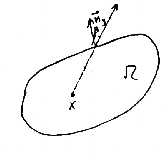
\includegraphics[width=0.2\textwidth]{31_2_new}
\end{center}
\begin{lemma}
Пусть $\Omega$ - ограниченная область с границей $G \in C^2, u(x) \in C^2(\Omega) \cap C(\bar{\Omega})$, а у $u(x) \Exists $ ПНП по направлению внешней нормали $\vec{n}(x^o), \Delta u \in C(\Omega)$. Тогда $$\int_{\Omega} (\Delta u)udx = \oint_{\Gamma} \frac{\partial u}{\partial \vec{n}}(x) u(x)dS - \int_{\Omega} |\triangledown|^2 dx $$
\end{lemma}
\begin{proof}
$u(x) \in C^2(\Omega) \cap C(\bar{\Omega}) => u(x) \in C^2(\Omega_{\delta}) \cap C^1(\Omega_{\delta}) => $

$$\int_{\Omega_{\delta}}(\Delta u(x))u(x)dx (1) = \oint_{G_{\delta}} \frac{\partial u}{\partial \vec{n}}u(x)dS (2) - \int_{\Omega_{\delta}}|\triangledown u(x)|^2dx (3)$$

$\lim_{\delta \to 0}(1) = \int_{\Omega} \Delta udx$, т.к. $\Delta u(x)$ и $u(x) \in C(\bar{\Omega})$

$\lim_{\delta \to 0}(2) = \int_{G_{\delta}} \frac{\partial u}{\partial \vec{n}}u(x)dS $

$\lim_{\delta \to 0}(3) = \lim_{x = x^o - \delta \vec{n}x^o} \int_{\Omega_{\delta}} |\triangledown u(x)|^2dx$

$\bullet$ С учетом сделанного обобщения все сделанные ранее рассуждения о внутренних и внешних задачах верны и для расширенного понятия классического решения.
\end{proof}
\begin{theorem}[Кореектная постановка внутренней задачи Неймана для уравнения Лапласа]
$\Omega$ - ограниченная область, граница $G \in C^2$. Найти функцию $u(x) \in C^2(\Omega) \cap C(\bar{\Omega})$, имеющую ПНП и удовлетворяющую 

\begin{equation}
\begin{cases}
\Delta u(x) = 0, x \in \Omega
\\
\frac{\partial u}{\partial \vec{n}}|_G = u_1(x) \in C(G)
\end{cases}
\end{equation}
\end{theorem}
\begin{theorem}[Корректная постановка внешней задачи Неймана для уравнения Лапласа]
$\Omega$ - внешняя область, граница $G \in C^2$. Найти функцию $u(x) \in C^2(\Omega) \cap C(\bar{\Omega})$ имеющую ПНП и удовлетворяющую 
\begin{equation}
\begin{cases}
\Delta u(x) = 0, x \in \Omega
\\
\frac{\partial u}{\partial \vec{n}}|_{\Gamma} = u_1(x) \in C(\Gamma)
\\
u(x)_{x \to \infty} \to 0
\end{cases}
\end{equation}
\end{theorem}
$\bullet$ Рассмотрим потенциал простого слоя

$\Omega$ - ограниченная область с границей $\Gamma \in C^2; x = x^o - \delta \vec{n}(x^o); 0 < \delta < \delta^*$
  $$V^* = \int_{\Gamma} \frac{\mu(x)}{|x - y|}dS_y$$

$$\frac{\partial u}{\partial \vec{n}}(x) = \sum_{k = 1}^3 n_k(x^o) \frac{\partial}{\partial x_k}\oint_{\Gamma} \frac{\mu(x)}{|x - y|}dS_y = \sum_{k = 1}^3 n_k(x^o) \frac{\partial}{\partial x_k}\oint_G \frac{1}{|x - y|}\mu(y)dS_y$$

$$\sum_{k = 1}^3 n_k(x^o) \frac{\partial}{\partial x_k} \frac{1}{|x - y|}\mu(y)dS_y = \oint_{\Gamma} \sum_{k = 1}^3 n_k(x^o) \frac{y_k - x_k}{|x - y|^3}\mu(y)dS_y = \oint_{\Gamma} \frac{(y - x, \vec{n}(x^o))}{|x - y|^3}\mu(y)dS_y$$

Обозначим $\left( \frac{\partial V^o}{\partial \vec{n}} \right)_{\pm}(x^o) = \lim_{x = x^o \mp \delta \vec{n}(x)}, \delta \to +0 \frac{\partial V^o}{\partial \vec{n}(x^o)} (x)$

$\frac{\partial V^o)}{\partial \vec{n}}(x^o)(1) = \int_{\Gamma} \frac{(y - x^o, \vec{n}(x^o))}{|x^o - y|^3}\mu(y)dS_y, x^o \in G(2)$

(1) - прямое значение нормальной производной

(2) - полярное ядро => $\forall \mu(x) \in C(G), \Forall x^o \in \Gamma$ этот интеграл существует, и более того $(1) \in C(\Gamma)$

\begin{theorem}
У потенциала простого слоя $V^o(x)$ с плотностью $\mu(x) \in C(\Gamma)$ существует ПНП на $\Gamma$: $$\left( \frac{\partial V^o}{\partial \vec{n}}_+(x^o)\right)
\text{и} \left(\frac{\partial V^o}{\partial \vec{n}}_-(x^o) \right),$$
причем имеет место формула скачка 

$$\left(\frac{\partial V^o}{\partial \vec{n}}_{\pm}(x^o) \right) = \frac{\partial V^o}{\partial \vec{n}}(x^o) \pm 2\pi \mu(x^o) $$
\end{theorem}
\begin{conseq}
$\left(\frac{\partial V^o}{\partial \vec{n}} \right)_+(x^o) - \left(\frac{\partial V^o}{\partial \vec{n}} \right)_-(x^o) = 4\pi \mu(x^o), x^o \in \Gamma$

$\frac{\partial V^o}{\partial \vec{n}}(x^o) = \frac{1}{2} \left[ \left(\frac{\partial V^o}{\partial \vec{n}} \right)_+(x^o) + \left(\frac{\partial V^o}{\partial \vec{n}} \right)_=(x^o)\right], x \in \Gamma$
\end{conseq}
